% !Mode:: "TeX:UTF-8"

% ---------- 声明文档类 ---------- %
% 有三个非官方的可选参数:coverpage, bindingpage, titlepage
% 分别表示显示封面页、显示装订页、显示标题页
% 删掉参数即表示该页不显示
%\documentclass[coverpage, bindingpage, titlepage]{dlmubachelorthesis}
\documentclass[coverpage]{dlmubachelorthesis}
% ================================================== %


% --------------- 添加批注 --------------- %
\let\comment\undefined
\usepackage[]{changes}
\definechangesauthor[name={海哥}, color=blue]{海哥} %创建批注者信息
\definechangesauthor[name={海老}, color=red]{海老} %创建批注者信息
% ======================================== %


% -------------------- 填写论文信息 -------------------- %
\cntitle{基于低分辨率视频的手势运动方向检测} %【中文标题】
\entitle{Detection of Gesture Motion Direction based on Low-Resolution Video} %【英文标题】
\aauthor{海哥} %【作者姓名】
\sdtID{222020xxxx} %【学号】
\faculty{理学院} %【学院】
\majorinCOVERPAGE{数学与应用数学2020-1} %【专业年级班级(coverpage专用)】
\majorinTITLEPAGE{数学与应用数学1班} %【专业班级(titlepage专用)】
\mentorONE{海老}{教授} %【指导教师(及其职称)】
\mentorTWO{无}{0} %【第二指导教师(及其职称)】【若无,则第一个参数填“无”,第二个填数字0】
\completiondate{2024}{5} %【完成日期(年、月)】
% ================================================== %


% ---------- 可以在此处添加自己定义的命令 ---------- %

% ================================================== %


\begin{document}

\makepages %【添加封面页、装订页、标题页】

\pagestyle{plain} %从摘要到目录,设置为无页眉、有页脚的模式
\pagenumbering{Roman} %《手册》要求:从摘要到目录,设置罗马数字页码
\renewcommand{\baselinestretch}{1.25}

% ---------- 中文摘要 ---------- %
\begin{abstract}

% ---------- 中文摘要内容 ---------- %
{\zihao{-4} %【该句涉及到格式设置,请勿乱动】

本文针对手机摄像头所获取的视频文件,进行手势运动方向的检测。针对低端摄像头视频图像的特点,本文采用了基于背景去除和肤色模型的方法对手部区域进行检测,并判别手部运动的方向。

首先,获取视频图像序列,即从视频文件中获取每一帧图像作为待检测的视频图像序列;其次,对获取的视频图像序列中的每一帧图像进行颜色模型转换、背景去除、图像二值化、形态学处理等预处理;然后,利用区域增长方法来检测视频图像序列中的手部连通区域,并计算每帧图像中手部区域的中心;最后根据图像序列中手部区域中心位置的变化来判断手部运动方向。

本文在Visual c++6.0开发环境下,借助于OpenCV开放平台,设计并实现了基于低端摄像头视频手势运动检测系统,得到了较好的检测效果。


\keywordsCN{运动目标检测;颜色模型;区域增长}
} 
\end{abstract}
% ================================================== %	

\newpage

% ---------- 英文摘要 ---------- %
\renewcommand\abstractname{\large ABSTRACT} %临时修改摘要名
\begin{abstract}

% ---------- 英文摘要内容 ---------- %
{\zihao{-4} %【该句涉及到格式设置,请勿乱动】

In this paper, the detection of hand motion direction is performed for the video files acquired by cell phone camera. Aiming at the characteristics of low-end camera video images, this paper adopts a method based on background removal and skin color model to detect the hand region and to discriminate the direction of hand motion.

Firstly, a video image sequence is acquired, i.e., each frame from the video file is acquired as a video image sequence to be detected; secondly, each frame in the acquired video image sequence is preprocessed with color model conversion, background removal, image binarization, morphological processing, etc.; then, a region growing method is used to detect the hand connectivity region in the video image sequence and to calculate the center of the hand region in each frame; finally, the hand region is detected based on the color model in the image sequence and the direction of hand movement is detected based on the color model. The center of the hand region; finally, the hand movement direction is judged based on the change of the center position of the hand region in the image sequence.

In this paper, under Visual c++6.0 development environment, with the help of OpenCV open platform, we designed and realized the hand gesture motion detection system based on low-end camera video, and got a better detection effect.

\keywordsEN{Moving Target Detection; Color Model; Regional Growth}
} 
\end{abstract}
% ================================================== %	

\newpage

% ---------- 目录 ---------- %
\tableofcontents
\listofchanges
\newpage
% ================================================== %	

\pagestyle{fancy} %从第一章到致谢,设置为有页眉、有页脚的模式
\pagenumbering{arabic} %《手册》要求:从正文开始设为阿拉伯数字页码,并且重新从1开始计数

% ---------- 正文首页标题 ---------- %
\cntitleinMAINBODY %【插入中文标题】
% ================================================== %


% ---------- 正文(划分为多个独立文件依次导入) ---------- %

\section{绪论}

本模板只是作为本科论文格式示例作用,为尽可能涵盖《毕业论文撰写规范》规定的内容,部分图片或表格与论文内容无关,该模板论文无研究意义,师生只做格式参考。

\subsection{课题研究的背景及意义}

摄像头(camera)又称为电脑相机、电脑眼等,它作为一种视频输入设备,在过去被广泛的运用于视频会议、远程医疗及实时监控等方面。近些年来,随着互联网技术的发展,网络速度的不断提高,再加上感光成像器件技术的成熟,使得摄像头得到了越来越广泛的应用。

\subsubsection{视频运动目标检测的研究现状}

视频序列中运动目标的检测与跟踪是计算机视觉和图像编码研究领域的一个重要课题,在机器人导航、智能监视系统、交通检测、医学图像处理以及视频图像压缩和传输等领域都有广泛的应用。运动目标检测就是判断视频序列中是否存在运动目标,并确定运动目标的位置。运动目标的提取主要包括运动检测以及目标提取两个步骤,其中运动检测处于整个视觉监视系统的最底层,是各种后续高级处理如目标分类,行为理解等的基础。

在近年来,随着技术的快速发展,多领域的研究都取得了显著的进展。特别是在数据处理、目标检测以及环境科学等领域,新的理论和方法不断涌现,为解决实际问题提供了有力的支持。

首先,在数据处理和导航系统的应用方面,付梦印等人深入探讨了Kalman滤波理论及其在导航系统中的应用\upcite{付梦印2003}。Kalman滤波作为一种高效的递归滤波器,通过预测和更新两个步骤,能够在存在不确定性的动态系统中估计出系统状态。这一理论在导航系统中的应用,极大地提高了系统的准确性和可靠性。

在目标检测领域,邓宇的研究为我们提供了复杂背景下运动目标检测技术的深入见解\upcite{邓宇2007}。随着计算机视觉和图像处理技术的不断发展,目标检测技术在安防、交通监控等领域的应用越来越广泛。如何在复杂的背景下准确、快速地检测出目标,成为该领域的重要研究方向。

在环境科学领域,张爱茜等人关注了氯代芳香族化合物对羊角月牙藻的毒性及QSAR分析\upcite{张爱茜2000}。这一研究不仅揭示了氯代芳香族化合物对水生生物的潜在危害,还通过QSAR(定量结构-活性关系)分析,为预测和评估这类化合物的环境风险提供了有力的工具。

此外,文献\cite{Stauffer1999}提出了自适应背景混合模型(Adaptive Background Mixture Models),为实时跟踪提供了新的解决方案。这一模型通过对背景图像进行建模和更新,能够有效地区分前景目标和背景,为视频监控、人机交互等领域的研究提供了新的思路。

综上所述,从Kalman滤波理论在导航系统中的应用,到复杂背景下的目标检测技术,再到环境科学中的毒性评估和QSAR分析,以及实时跟踪中的自适应背景混合模型,这些研究成果不仅丰富了相关领域的理论和方法,也为解决实际问题提供了有力的支持。随着技术的不断进步,相信这些领域的研究将会取得更加显著的成果。

\subsubsection{运动目标检测技术}

运动目标检测技术研究如何完成研究对象(图像序列)中感兴趣的目标区域的“准确定位”问题。

\fourthsection{帧间差分法}

三种传统的运动目标检测算法之一。帧间差分式检测相邻两帧图像之间变化的最简单、最直接的方法,它是直接比较了两帧图像对应像素点的灰度值的不同,然后通过阈值来提取序列图像中的运动区域。二值图像中为“$0$”的像素对应在前后两帧图像之间没有发生(由于运动而产生的)变化的地方,为“1”的像素对应两帧图像间发生变化的地方,这常是由目标运动而产生的。

计算得到
\begin{equation}%\label{}
Q_s = \varphi(h-z)^{3/2}F^{4/5}\beta\gamma\delta,
\end{equation}
其中,$E_s$与$E_c$分别表示基体和涂层的平均弹性模量;$\alpha_s$与$\alpha_c$分别表示基体和涂层的热膨胀系数;$\Delta T$表示喷涂前后温差;$D$与$d$分别表示基体和涂层的厚度。

将所查各值代入公式可得:
\begin{align}%\label{}
  C_0 &= \sqrt{ 2\frac{k}{k-1}RT_0^{\ast}\lt(1-\frac{1}{\prod_{T}^{m}}\rt) } \notag \\
   &= \sqrt{ 2\times \frac{1.4}{1.4-1}\times 287\times 285\times \lt( 1-\frac{1}{3^{0.286}} \rt) } \notag \\
   &= 392.9~\unit{m/s}.
\end{align}

处理过程如图\ref{fig:手部运动方向检测结构图}所示。
\begin{figure}[H]
  \centering
  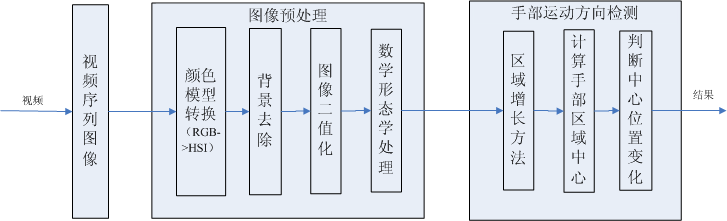
\includegraphics[width=0.8\textwidth]{fig_ch1/手部运动方向检测结构图.png}
  \caption{手部运动方向检测结构图}
  \label{fig:手部运动方向检测结构图}
\end{figure}

由图\ref{fig:手部运动方向检测结构图}可以知道,当得到一个变量的概率密度函数pdf时,熵就可以用来度量其状态的连贯性,同时,熵也是能量的一种表示。

\subsection{本章小结}

视频序列中运动目标的检测与跟踪是计算机视觉和图像编码研究领域的一个重要课题,在机器人导航、智能监视系统、交通检测、医学图像处理以及视频图像压缩和传输等领域都有广泛的应用。运动目标检测就是判断视频序列中是否存在运动目标,并确定运动目标的位置。 \clearpage\vspace*{0pt} %\vspace*{0pt}的添加解决了章节标题前间距不合理的问题

\section{基础知识}

基于视频序列的运动目标检测与跟踪涉及到很多研究领域,如数字图像处理、计算机视觉、信息融合、模式识别与人工智能等。

\subsection{视频图像预处理}

\subsubsection{常用颜色模型}

颜色模型的用语是在某些标准下用通常可接受的方式简化彩色规范。本质上颜色模型是坐标系统和子空间的规范。位于系统中的每种颜色都由单个点来表示。

(1)~RGB彩色模型:

在RGB模型中,每种颜色出现在红、绿、蓝的原色光谱分量中,这个模型基于笛卡尔坐标系。

图\ref{fig:RGB彩色立方体示意图}所示的立方体。图中R、G、B位于$3$个角上。在该模型中,灰度等级沿着主对角线从原点的黑色到点$(1,1,1)$的白色分布。
\begin{figure}[H]
  \centering
  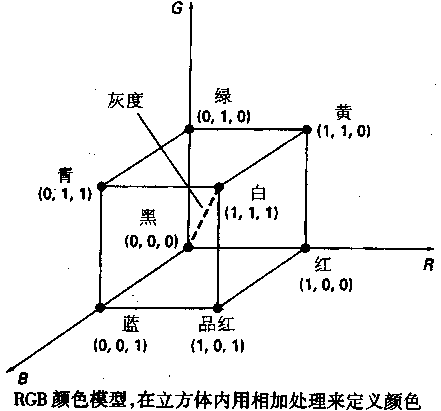
\includegraphics[width=0.45\textwidth]{fig_ch2/RGB彩色立方体示意图.png}
  \caption{RGB彩色立方体示意图}
  \label{fig:RGB彩色立方体示意图}
\end{figure}

(2)~灰色模型:

本质上颜色模型是坐标系统和子空间的规范。位于系统中的每种颜色都由单个点来表示。单位在每列的书写示例如表\ref{tab:单位在每列的书写示例}所示。

\begin{table}[H]
  \centering
  \caption{单位在每列的书写示例}
    \begin{tabular}{ccccc}
    \toprule
    基体 & 序号 & \makecell[c]{粉末类型和\\ 预热温度(\unit{\degreeCelsius})} & 失效温度(\unit{\degreeCelsius}) & $E_c$计算值(\unit{\GPa})\\
    \midrule
    \multicolumn{1}{c}{\multirow{4}[2]{*}{SUS304不锈钢}} & 1     & 粗粉 \& 1000 & 180   & 4.21 \\
          & 2     & 粗粉 \& 800 & 10    & 4.38 \\
          & 3     & 细粉 \& 1000 & 300   & 4.95 \\
          & 4     & 细粉 \& 800 & 120   & 5.08 \\
    \bottomrule
    \end{tabular}%
  \label{tab:单位在每列的书写示例}%
\end{table}%

表格的分栏情况示例如表\ref{tab:分栏情况示例}所示。
% Table generated by Excel2LaTeX from sheet 'Sheet1'
\begin{table}[H]
  \centering
  \caption{分栏情况示例}
    \begin{tabular}{cccc}
    \toprule
    \multicolumn{1}{c}{基体} & 粉末类型 & \multicolumn{1}{c}{预热温度(\unit{\degreeCelsius})} & \multicolumn{1}{c}{平均值} \\
    \midrule
    \multicolumn{1}{c}{\multirow{6}[4]{*}{SUS304不锈钢}} & \multirow{3}[2]{*}{粗粉} & 600   & 44.28\% \\
          & \multicolumn{1}{c}{} & 800   & 42.37\% \\
          & \multicolumn{1}{c}{} & 1000  & 39.74\% \\
\cmidrule{2-4}          & \multirow{3}[2]{*}{细粉} & 600   & 27.95\% \\
          & \multicolumn{1}{c}{} & 800   & 25.41\% \\
          & \multicolumn{1}{c}{} & 1000  & 24.77\% \\
    \midrule
    \multicolumn{1}{c}{\multirow{2}[2]{*}{碳钢}} & 粗粉    & 1000  & 35.65\% \\
          & 细粉    & 1000  & 22.95\% \\
    \bottomrule
    \end{tabular}%
  \label{tab:分栏情况示例}%
\end{table}%

表的通栏情况和全表统一单位的情况如表\ref{tab:插入表格的通栏示例(单位:台)}所示。
% Table generated by Excel2LaTeX from sheet 'Sheet1'
\begin{table}[htbp]
  \centering
  \caption{插入表格的通栏示例(单位:台)}
    \begin{tabular}{cccc}
    \hline%\toprule
    \diagbox{时间}{地点} & 电风扇 & 冰箱 & 洗衣机 \\
    \hline%\midrule
    10月   & 100   & 200   & 300 \\
    11月   & 200 & & \\
    12月   & 200 & 100   & 400 \\
    \hline%\midrule
    合计    & 500   & 500   & 900 \\
    \hline%\bottomrule
    \end{tabular}%
  \label{tab:插入表格的通栏示例(单位:台)}%
\end{table}%

{\color{red}\lipsum[4]} %添加这么一段测试文本是为了展示跨页表格的效果

若表格一页内放不下,可以使用跨页表格。跨页表格的情况如表\ref{tab:CMS_VIDEO数据表(跨页表格)}所示。
\begin{longtable}{ccccc}
    \caption{CMS\_VIDEO数据表(跨页表格)} \label{tab:CMS_VIDEO数据表(跨页表格)} \\
	\toprule
	字段标识 & 字段含义 & 数据类型 & 是否主键 & 是否外键 \\
	\midrule
    \endfirsthead %以上是首页表头
    \caption{(续表)} \\ %续表对应的标题
    \midrule
    字段标识 & 字段含义 & 数据类型 & 是否主键 & 是否外键 \\
    \midrule
    \endhead %以上是通用表头
    \midrule
    \endfoot %以上是通用表尾
    \bottomrule
    \endlastfoot %以上是末页表尾,以下是表格正文
    ID & ID & INTEGER & 是 & 否 \\
    VIDEO\_NAME & 视频名称 & VARCHAR2($20$) & 否 & 否 \\
    VIDEO\_TYPE & 视频类型 & VARCHAR2($20$) & 否 & 是 \\
    VIDEO\_PATH & 视频路径 & VARCHAR2($20$) & 否 & 否 \\
    UPLOADER\_ID & 上传人ID & INTERGER & 否 & 是 \\
    UPLOAD\_DATE & 上传日期 & DATE & 否 & 否 \\
    ISPASS & 是否审批 & INTERGER & 否 & 否
\end{longtable}

\subsection{本章小结}

本章主要介绍了表格的显示。 \clearpage\vspace*{0pt}

\section{视频图像预处理}

\subsection{引言}

本章是视频图像的预处理阶段,首先,获取视频图像;然后对视频图像序列中的每帧图像进行图像预处理。如图\ref{fig:手势运动方向检测流程图}所示。
\begin{figure}[H]
  \centering
  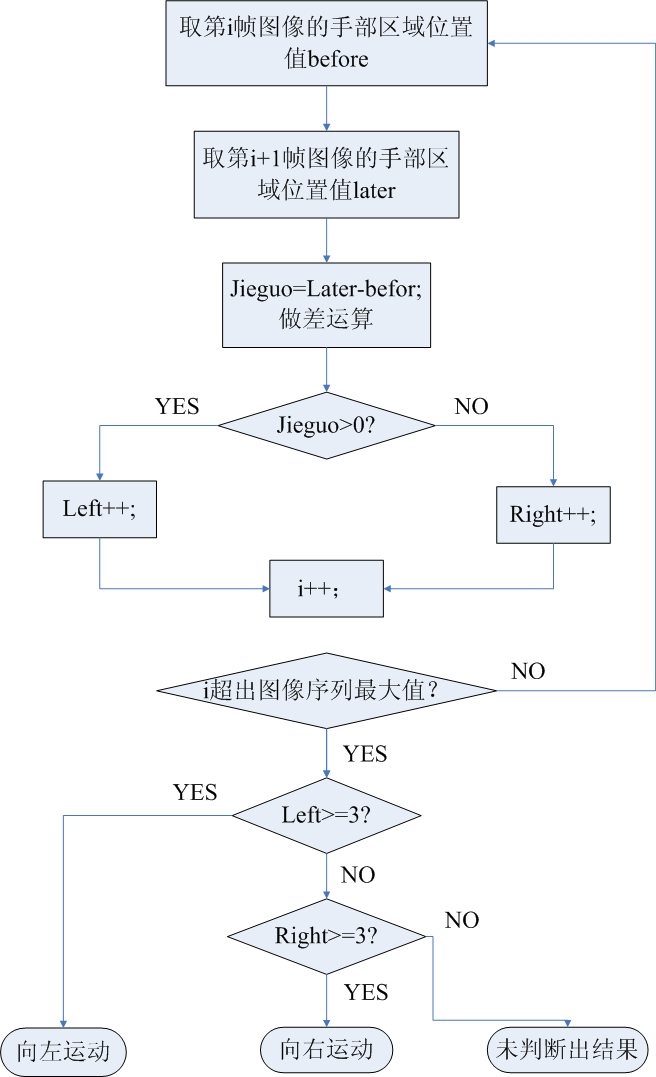
\includegraphics[width=0.5\textwidth]{fig_ch3/手势运动方向检测流程图.png}
  \caption{手势运动方向检测流程图}
  \label{fig:手势运动方向检测流程图}
\end{figure}

由图\ref{fig:手势运动方向检测流程图}可知,视频图像的预处理阶段,首先,获取视频图像;然后对视频图像序列中的每帧图像进行图像预处理。

\subsection{图像的多种显示方式}

分图的情况如图\ref{fig:涂层在冷却过程中残余热应力的变化情况}所示。
\begin{figure}[H]
    \centering
    \begin{minipage}[c]{0.48\textwidth}
        \centering
        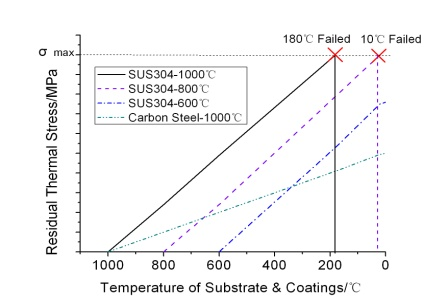
\includegraphics[height=0.2\textheight]{fig_ch3/粗粉_涂层在冷却过程中残余热应力的变化情况.png}
        \subcaption{粗粉涂层}
    \end{minipage}
    \begin{minipage}[c]{0.48\textwidth}
        \centering
        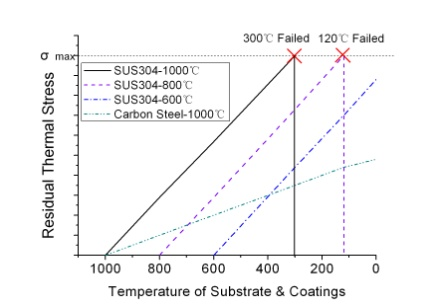
\includegraphics[height=0.2\textheight]{fig_ch3/细粉_涂层在冷却过程中残余热应力的变化情况.png}
        \subcaption{细粉涂层}
    \end{minipage}
    \caption{涂层在冷却过程中残余热应力的变化情况}\label{fig:涂层在冷却过程中残余热应力的变化情况}
\end{figure}

在图中说明比较多的情况下,采取如图\ref{fig:透平膨胀机的组成结构}的格式。
\begin{figure}[H]
  \centering
  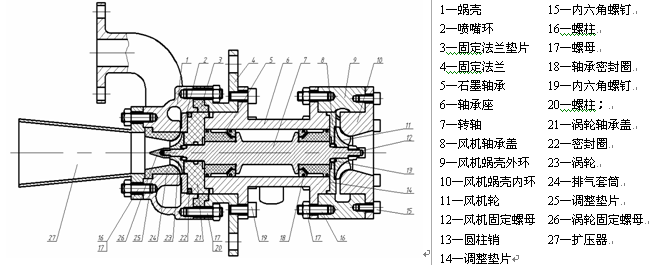
\includegraphics[width=0.7\textwidth]{fig_ch3/透平膨胀机的组成结构.png}
  \caption{透平膨胀机的组成结构}
  \label{fig:透平膨胀机的组成结构}
\end{figure}

\subsection{本章小结}

本章主要介绍了图片的格式。

 \clearpage\vspace*{0pt}

\section{系统性能分析}

{\bf 伪代码的使用示例如下所示。}

\begin{algorithm}
\SetKwData{Left}{left}\SetKwData{This}{this}\SetKwData{Up}{up} % 定义快捷变量,后续使用时只需:反斜杠+变量名
\SetKwFunction{Union}{Union}\SetKwFunction{FindCompress}{FindCompress} % 定义函数,后续使用时只需:反斜杠+函数名
\SetKwInOut{Input}{输入}\SetKwInOut{Output}{输出} %此处可自定义输入、输入的名称格式

在此处添加不带编号的内容(若无,则将该行注释即可)。\\
\LinesNumbered % 使下列算法描述带行号
\Input{A bitmap $Im$ of size $w\times l$} % 输入
\Output{A partition of the bitmap} % 输出
\BlankLine

\emph{special treatment of the first line}\;
\For{$i\leftarrow 2$ \KwTo $l$}{
  \emph{special treatment of the first element of line $i$}\;
  \For{$j\leftarrow 2$ \KwTo $w$}{\label{forins}
    \Left$\leftarrow$ \FindCompress{$Im[i,j-1]$}\;
    \Up$\leftarrow$ \FindCompress{$Im[i-1,]$}\;
    \This$\leftarrow$ \FindCompress{$Im[i,j]$}\;
    \If( \tcp*[h]{此处添加注释:O(\Left,\This)==1} ){\Left compatible with \This}{\label{lt} % \tcp*[h]{...}表示非对齐的注释
      \lIf{\Left $<$ \This}{\Union{\Left,\This}} %含else...的if语句用命令\lIf
      \lElse{\Union{\This,\Left}}
    }
    \If(\tcp*[f]{O(\Up,\This)==1}){\Up compatible with \This}{\label{ut} % \tcp*[f]{...}表示居右对齐的注释
      \lIf(\tcp*[f]{再次用Union函数}){\Up $<$ \This}{\Union{\Up,\This}}
      \tcp{\This is put under \Up to keep tree as flat as possible}\label{cmt} % \tcp{...}表示行内的注释
      \lElse{\Union{\This,\Up}}\tcp*[h]{\This linked to \Up}\label{lelse}
    }
  }
  \lForEach{element $e$ of the line $i$}{\FindCompress{p}}
}
\caption{不相交分解(disjoint decomposition)}\label{pcode: 不相交分解} %伪代码对应算法的标题及其引用标签
\end{algorithm}

引用时的格式为:算法\ref{pcode: 不相交分解}实现了...。

{\bf 下面用于展示基于\verb|changes|宏包的批注功能。}

北冥有鱼,其名为鲲。鲲之大,不知其几千里也;化而为鸟,其名为鹏。鹏之背,不知其几千里也;怒而飞,其翼若垂天之云。\added[id=海哥, comment={少了一句}]{是鸟也,海运则将徙于南冥。}南冥者,天池也。《齐谐》者,志怪者也。《谐》之言曰:“鹏之徙于南冥也,水击三千里,抟扶摇而上者九万里,去以六月息者也。”野马也,尘埃也,生物之以息相吹也。\deleted[id=海哥, comment={这句话删掉}]{之乎者也。}天之苍苍,其正色邪?其远而无所至极邪?其视下也,亦若是则已矣。且夫水之积也不厚,则其负大舟也无力。覆杯水于\replaced[id=海老, comment={用错词}]{坳堂}{水堂}之上,则芥为之舟,置杯焉则胶,水浅而舟大也。风之积也不厚,则其负大翼也无力。故九万里,则风斯在下矣,而后乃今培风;背负青天,而莫之夭阏者,而后乃今将图南。蜩与学鸠笑之曰:“我决起而飞,抢榆枋而止,时则不至,而控于地而已矣,奚以之九万里而南为?”适莽苍者,三餐而反,腹犹果然;适百里者,宿舂粮;适千里者,三月聚粮。之二虫又何知!

小知不及大知,小年不及大年。奚以知其然也?朝菌不知晦朔,蟪蛄不知春秋,此小年也\deleted[id=海老]{,不亦乐乎}。楚之南有冥灵者,以五百岁为春,五百岁为秋;上古有大椿者,以八千岁为春,八千岁为秋,此大年也。而彭祖乃今以久特闻,众人匹之,不亦悲乎!汤之问棘也是已。穷发之北,有冥海者,天池也。有鱼焉,其广数千里,未有知其修者,其名为鲲。有鸟焉,其名为鹏,背若泰山,翼若垂天之云,抟扶摇羊角而上者九万里,绝云气,负青天,然后图南,且适南冥也。斥鴳笑之曰:“彼且奚适也?我腾跃而上,不过数仞而下,翱翔蓬蒿之间,此亦飞之至也。而彼且奚适也?”此小大之辩也。

\highlight[id=海老]{故夫知效一官,行比一乡,德合一君,}而征一国者,其自视也,亦若此矣。而宋荣子犹然笑之。且举世誉之而不加劝,举世非之而不加沮,定乎内外之分,辩乎荣辱之境,斯已矣。彼其于世,未数数然也。虽然,犹有未树也。夫列子御风而行,泠然善也,旬有五日而后反。彼于致福者,未数数然也。此虽免乎行,犹有所待者也。\highlight[id=海老, comment={建议对其展开分析}]{若夫乘天地之正,而御六气之辩,以游无穷者,彼且恶乎待哉}?故曰:至人无己,神人无功,圣人无名\comment[id=海老]{建议把落款补上}。

\iffalse
只能用这个命令
来实现多行注释
\fi
 \clearpage\vspace*{0pt}

\section*{结论}
\addcontentsline{toc}{section}{结论} % 将该章标题手动添加到目录中

在Visual c++6.0开发环境下,借助于OpenCV开放平台,设计并实现了基于低端摄像头视频手势运动检测系统。
 \clearpage\vspace*{0pt} % 结论
% ================================================== %

% ---------- 参考文献 ---------- %
\addcontentsline{toc}{section}{参~ 考~ 文~ 献} %不能放在导言区
{\zihao{5} %【该句涉及到格式设置,请勿乱动】
\vspace*{0pt} %【该句涉及到格式设置,请勿乱动】
\bibliography{refs} %bib文件导入的形式生成参考文献列表
%\begin{thebibliography}{100}
%\bibitem{文献x标签}文献x信息
%\end{thebibliography}
}
\clearpage\vspace*{0pt} %【该句涉及到格式设置,请勿乱动】
% ================================================== %

% ---------- 致谢 ---------- %

\begin{center}
\bf\zihao{3} 致\hspace{2em}谢
\end{center}
\addcontentsline{toc}{section}{致\hspace{2em}谢} % 将该章标题手动添加到目录中

衷心的感谢数学专业各位老师,在大学学习期间,给予了我极大地鼓励和帮助,在学习上给予了我严谨、耐心的指导,在生活上给与了我亲切、热情的关怀。老师们渊博的学识、谦逊、谨慎的治学作风,一丝不苟、尽职尽责的工作态度以及正直的为人之道,都将是我终身受益,并激励我始终刻苦努力。在此,我向各位老师表示崇高的敬意和衷心的感谢!


% ================================================== %

% ---------- 附录 ---------- %

\clearpage\vspace*{0pt} %【该句涉及到格式设置,请勿乱动】

\pagestyle{plain} %《手册》要求:从附录页开始,去掉页眉

{\zihao{5} %【该句涉及到格式设置,请勿乱动】

\appendixsec{企业信息表}

\begin{longtable}{cccc}
    \caption{企业信息表} \label{tab:企业信息表} \\
	\toprule
	字段名称 & 中文描述 & 类型 & 长度 \\
	\midrule
    \endfirsthead %以上是首页表头
    \caption{(续表)} \\ %续表对应的标题
    \midrule
    字段名称 & 中文描述 & 类型 & 长度 \\
    \midrule
    \endhead %以上是通用表头
    \midrule
    \endfoot %以上是通用表尾
    \bottomrule
    \endlastfoot %以上是末页表尾,以下是表格正文
    ID & ID & NUMBER & 15 \\
    COMPANY\_ID & 公司ID & VARCHAR2 & 60 \\
    LOGISTER\_AGENT & 委托代理人 & VARCHAR2 & 60 \\
    SHORT\_NAME & 物流商简称 & VARCHAR2 & 60 \\
    BUSINESS\_FIELD & 行业类别 & VARCHAR2 & 10 \\
    WAY\_VEHICLE & 公路运输 & VARCHAR2 & 10 \\
    WAY\_TRAIN & 铁路运输 & VARCHAR2 & 10 \\
    WAY\_SHIP & 船舶运输 & VARCHAR2 & 10 \\
    WAY\_PIPELINE & 管道运输 & VARCHAR2 & 10 \\
    WAY\_CONTAINER & 集装箱运输 & VARCHAR2 & 10 \\
    WAY\_OTHERS & 其他运输方式 & VARCHAR2 & 60 \\
    FAX & 传真 & DATE & \\
    SETUP\_DATE & 成立日期 & VARCHAR2 & 60 \\
    BUSINESS\_LICENSECODE & 营业执照号码 & DATE & \_\_ \\
    BUSINESS\_LICENSEDATE & 营业执照有效期 & VARCHAR2 & 60 \\
    GAS\_LICENSECODE & 许可证号码 & DATE & \_\_ \\
    GAS\_LICENSEDATE & 许可证有效期 & VARCHAR2 & 60 \\
    HAZARD\_LICENSECODE & \makecell{化学危险品经营 \\ 许可证号码} & DATE & \_\_ \\
    HAZARD\_LICENSEDATE & \makecell{化学危险品经营 \\ 许可证有效期} & VARCHAR2 & 60 \\
    STATE\_TAXACCOUNT & 国税税号 & VARCHAR2 & 60 \\
    CREATE\_USERID & 创建人 & NUMBER & 15
\end{longtable}

\newpage

\appendixsec{程序代码}

%以文件形式插入代码
\lstinputlisting[ language=C++, title={\raggedright\normalsize 计算$\bk{n}$的阶乘(C++):} ]{codes/funfactorial.cpp} %C++

\lstinputlisting[ language=Java, title={\raggedright\normalsize 计算$\bk{n}$的阶乘(Java):} ]{codes/funfactorial.java} %Java

\lstinputlisting[ language=Python, title={\raggedright\normalsize 计算$\bk{n}$的阶乘(Python):} ]{codes/funfactorial.py} %Python

\lstinputlisting[style=Matlab-editor, title={\raggedright\normalsize 计算$\bk{n}$的阶乘(MATLAB):}]{codes/funfactorial.m} %MATLAB(如果不想要这种风格,则把该行命令的可选参数style=Matlab-editor改为language=Matlab


} %字号设置
% ================================================== %

\end {document} 